\documentclass[border=10pt]{standalone}

\usepackage{tikz}
\usepackage{tikzsymbols}
\usetikzlibrary{calc,patterns,shapes.geometric}

\def\centerarc[#1](#2)(#3:#4:#5){\draw[#1] ($(#2)+({#5*cos(#3)},{#5*sin(#3)})$) arc (#3:#4:#5);}

\begin{document}
	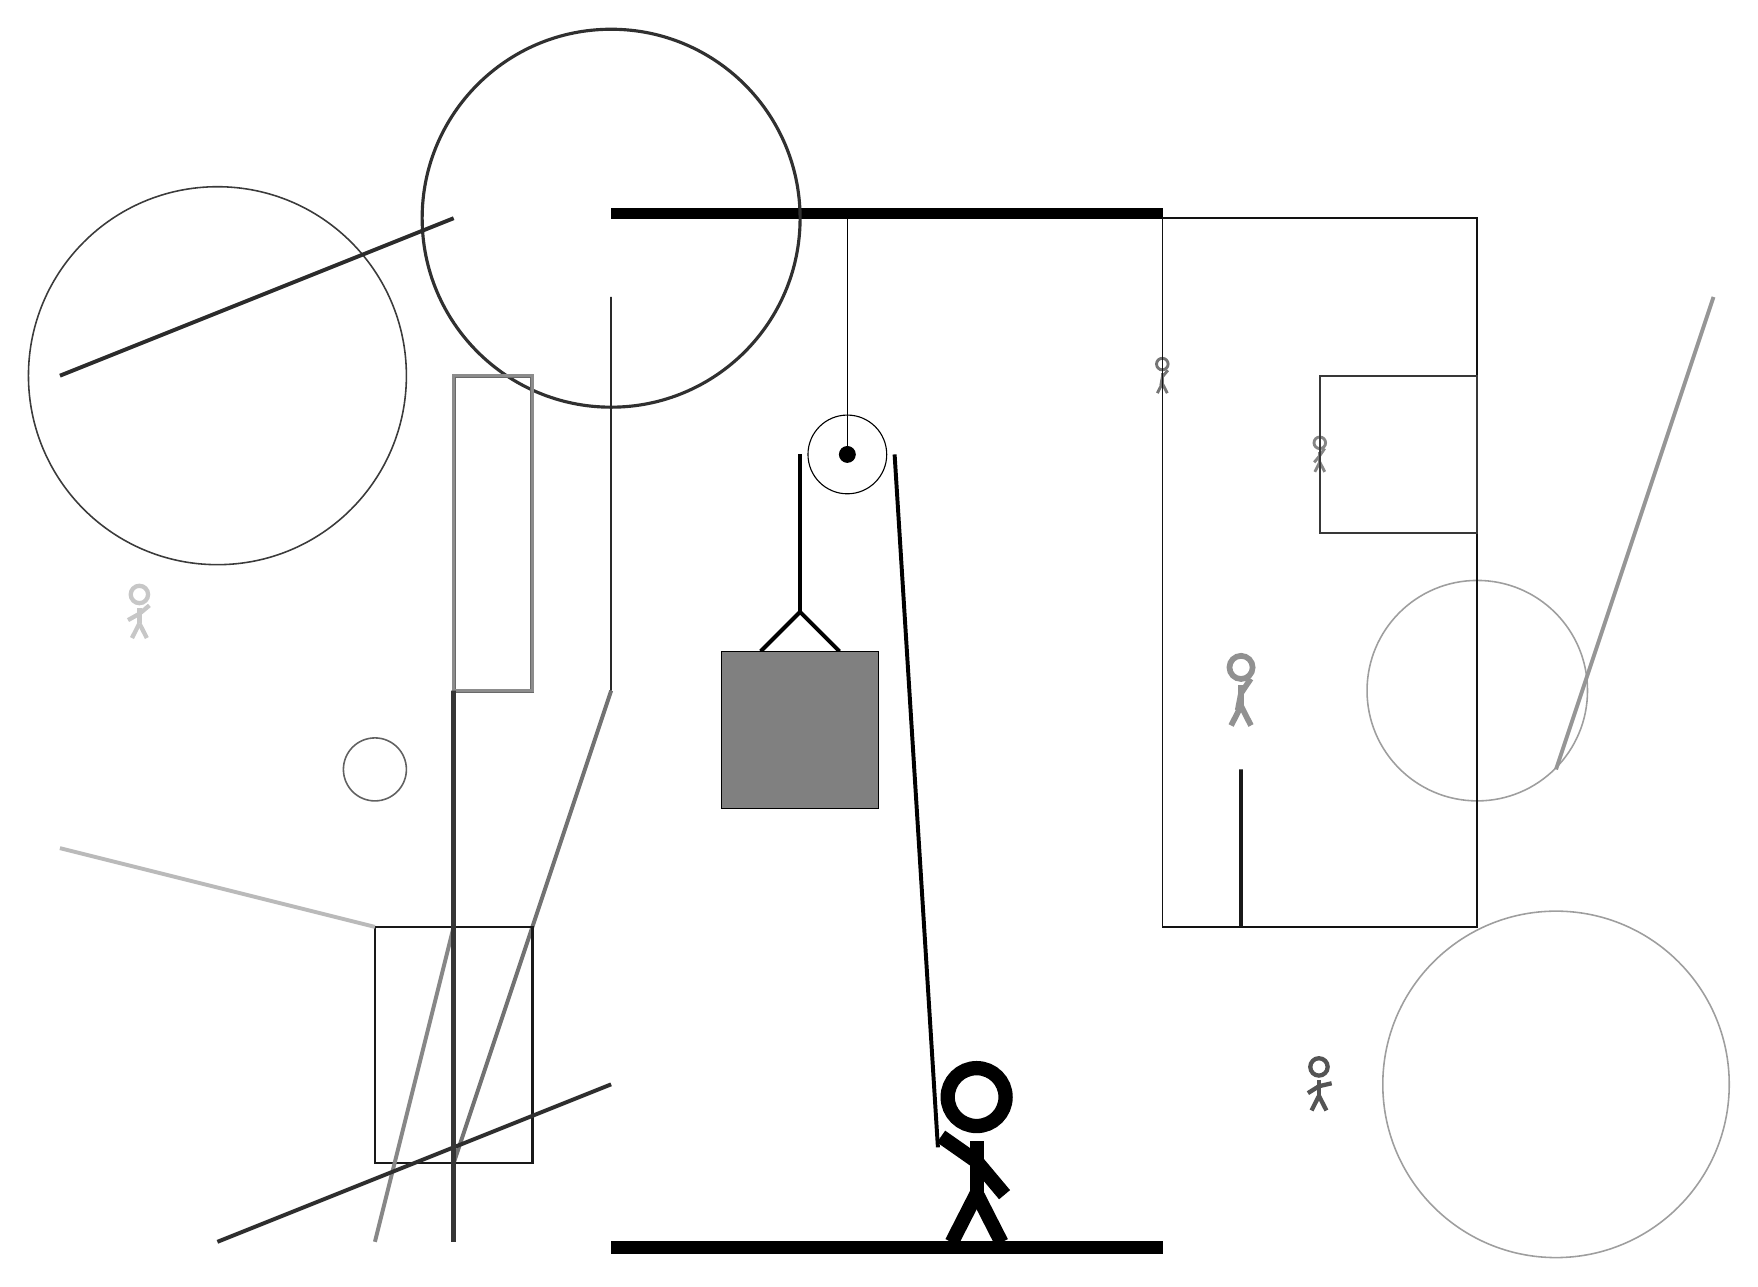
\begin{tikzpicture}
		%%%%% START %%%%%
		
		\draw[fill=black] (-2, 10) rectangle (5, 10.125);
		
		\draw (1, 7) circle (0.5);
		\draw[fill=black] (1, 7) circle (0.1);
		\draw (1, 10) -- (1, 7);
		
		\draw[line width=0.5mm] (-0.1, 4.5) -- (0.4, 5.0) -- (0.9, 4.5);
		\draw[fill=black!50] (-0.6, 4.5) rectangle (1.4, 2.5);
		
		\draw[line width=0.5mm] (0.4, 7) -- (0.4, 5.0);
		\centerarc[line width=0.5mm](1, 7)(0:180:0.6);
		\draw[line width=0.5mm](1.6, 7) -- (2.15, -1.8);
		
		\draw [line width=0.4mm, color=black!81](-2, 10) circle (2.4);
		
		\node[line width=0.4mm, color=black!54] at (5, 8) {\Strichmaxerl[2][80][50]};
		\draw [line width=0.6mm, color=black!35](9, 3) circle (0.0);
		\draw [line width=0.2mm, color=black!38](9, 4) circle (1.4);
		\node[line width=0.5mm, color=black!48] at (7, 7) {\Strichmaxerl[2][50][56]};
		\draw[line width=0.5mm, color=black!55](-4, -2) -- (-2, 4);
		
		\draw[line width=0.3mm, color=black!90] (-3, -2) rectangle (-5, 1);
		\draw [line width=0.2mm, color=black!77](-7, 8) circle (2.4);
		\draw[line width=0.5mm, color=black!20] (-3, 5) rectangle (-3, 6);
		\draw[line width=0.5mm, color=black!27](-5, 1) -- (-9, 2);
		\node[line width=0.7mm, color=black!43] at (6, 4) {\Strichmaxerl[4][79][56]};
		\draw[line width=0.5mm, color=black!47](-5, -3) -- (-4, 1);
		\node[line width=0.6mm, color=black!67] at (7, -1) {\Strichmaxerl[3][32][13]};
		
		\draw[line width=0.5mm, color=black!59] (-3, 8) rectangle (-4, 4);
		\draw[line width=0.2mm, color=black!93] (5, 1) rectangle (9, 10);
		\draw[line width=0.4mm, color=black!45] (-4, 4) rectangle (-3, 8);
		\node[line width=0.5mm, color=black!22] at (-8, 5) {\Strichmaxerl[3][29][40]};
		\draw[line width=0.5mm, color=black!82](-7, -3) -- (-2, -1);
		\draw[line width=0.3mm, color=black!78] (7, 8) rectangle (9, 6);
		
		\draw[line width=0.4mm, color=black!90] (6, 1) rectangle (6, 3);
		\draw[line width=0.2mm, color=black!84] (-2, 9) rectangle (-2, 4);
		
		\draw [line width=0.2mm, color=black!38](10, -1) circle (2.2);
		
		\draw[line width=0.5mm, color=black!83](-4, 10) -- (-9, 8);
		\draw[line width=0.6mm, color=black!79] (-4, -3) rectangle (-4, 4);
		\draw [line width=0.2mm, color=black!62](-5, 3) circle (0.4);
		
		\draw[line width=0.5mm, color=black!41](10, 3) -- (12, 9);
		
		\node at (2.6, -1.9) {\Strichmaxerl[10][-35][-50]};
		
		\draw[fill=black] (-2, -3) rectangle (5, -3.15);
		
		%%%%% END %%%%%
	\end{tikzpicture}
\end{document}